\chapter{\TextoIdioma{Fundamentação teórica}{Theoretical background}}
\label{cap:fundamentacao}
\section{\TextoIdioma{Estados e operadores}{States and operators}}
Um qubit puro é representado no espaço de Hilbert bidimensional por
\begin{equation}\label{eq:qubit}
  \lvert\psi\rangle=\alpha\lvert0\rangle+\beta\lvert1\rangle,
  \qquad |\alpha|^{2}+|\beta|^{2}=1.
\end{equation}
Estados gerais são representados por operadores densidade $\rho\succeq0$ com $\operatorname{Tr}\rho=1$. A entropia de von Neumann é
\begin{equation}\label{eq:entropia}
  S(\rho)=-\operatorname{Tr}\bigl(\rho\log_{2}\rho\bigr).
\end{equation}
A interpretação da compressão de informação quântica é discutida em \textcite{schumacher1995}. 

\section{\TextoIdioma{Representação esquemática}{Schematic representation}}
A Figura~\ref{fig:fluxo} apresenta um esquema simplificado de preparação e transformação de um estado.
\begin{figure}[htbp]
\centering
\caption{Esquema de preparação e transformação de um estado.}
\label{fig:fluxo}
\vspace{.35cm}
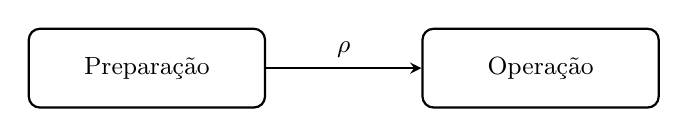
\begin{tikzpicture}[>=stealth,thick, every node/.style={font=\small}]
\node[draw,rounded corners,minimum width=3cm,minimum height=1cm] (a) at (0,0) {Preparação};
\node[draw,rounded corners,minimum width=3cm,minimum height=1cm] (b) at (5,0) {Operação};
\draw[->] (a) -- node[above] {$\rho$} (b);
\end{tikzpicture}
\par\medskip
\begin{minipage}{.55\textwidth}
\raggedright\footnotesize Fonte: elaboração própria.
\end{minipage}
\end{figure}
